\begin{atiTask}[
  title = Zweidimensionales Vektorfeld
  %call = Zusatzaufgabe,
]
Betrachten Sie das Vektorfeld
\[
\vec{V}=x^2y\vec{i}-x^3y^2\vec{j}\]
und den geschlossenen Weg $C$ entlang des Rechteckes $A(1,1)$, $B(3,1)$, $C(3,2)$ und $D(1,2)$.
\begin{atiSubtasks}
\item Berechnen Sie die Arbeit, die entlang des Weges $C$ in diesem Kraftfeld verrichtet wird, in dem Sie sowohl das Kurvenintegral, als auch das Flächenintegral berechnen [beide Seiten des \textsc{Green}schen Satzes].
\item Berechnen Sie den Fluss des Vektorfeldes durch die Kurve $C$, indem Sie beide Seiten des \textsc{Gauß}schen Satzes in der Ebene berechnen.
\end{atiSubtasks}
\end{atiTask}
\begin{atiSolution}
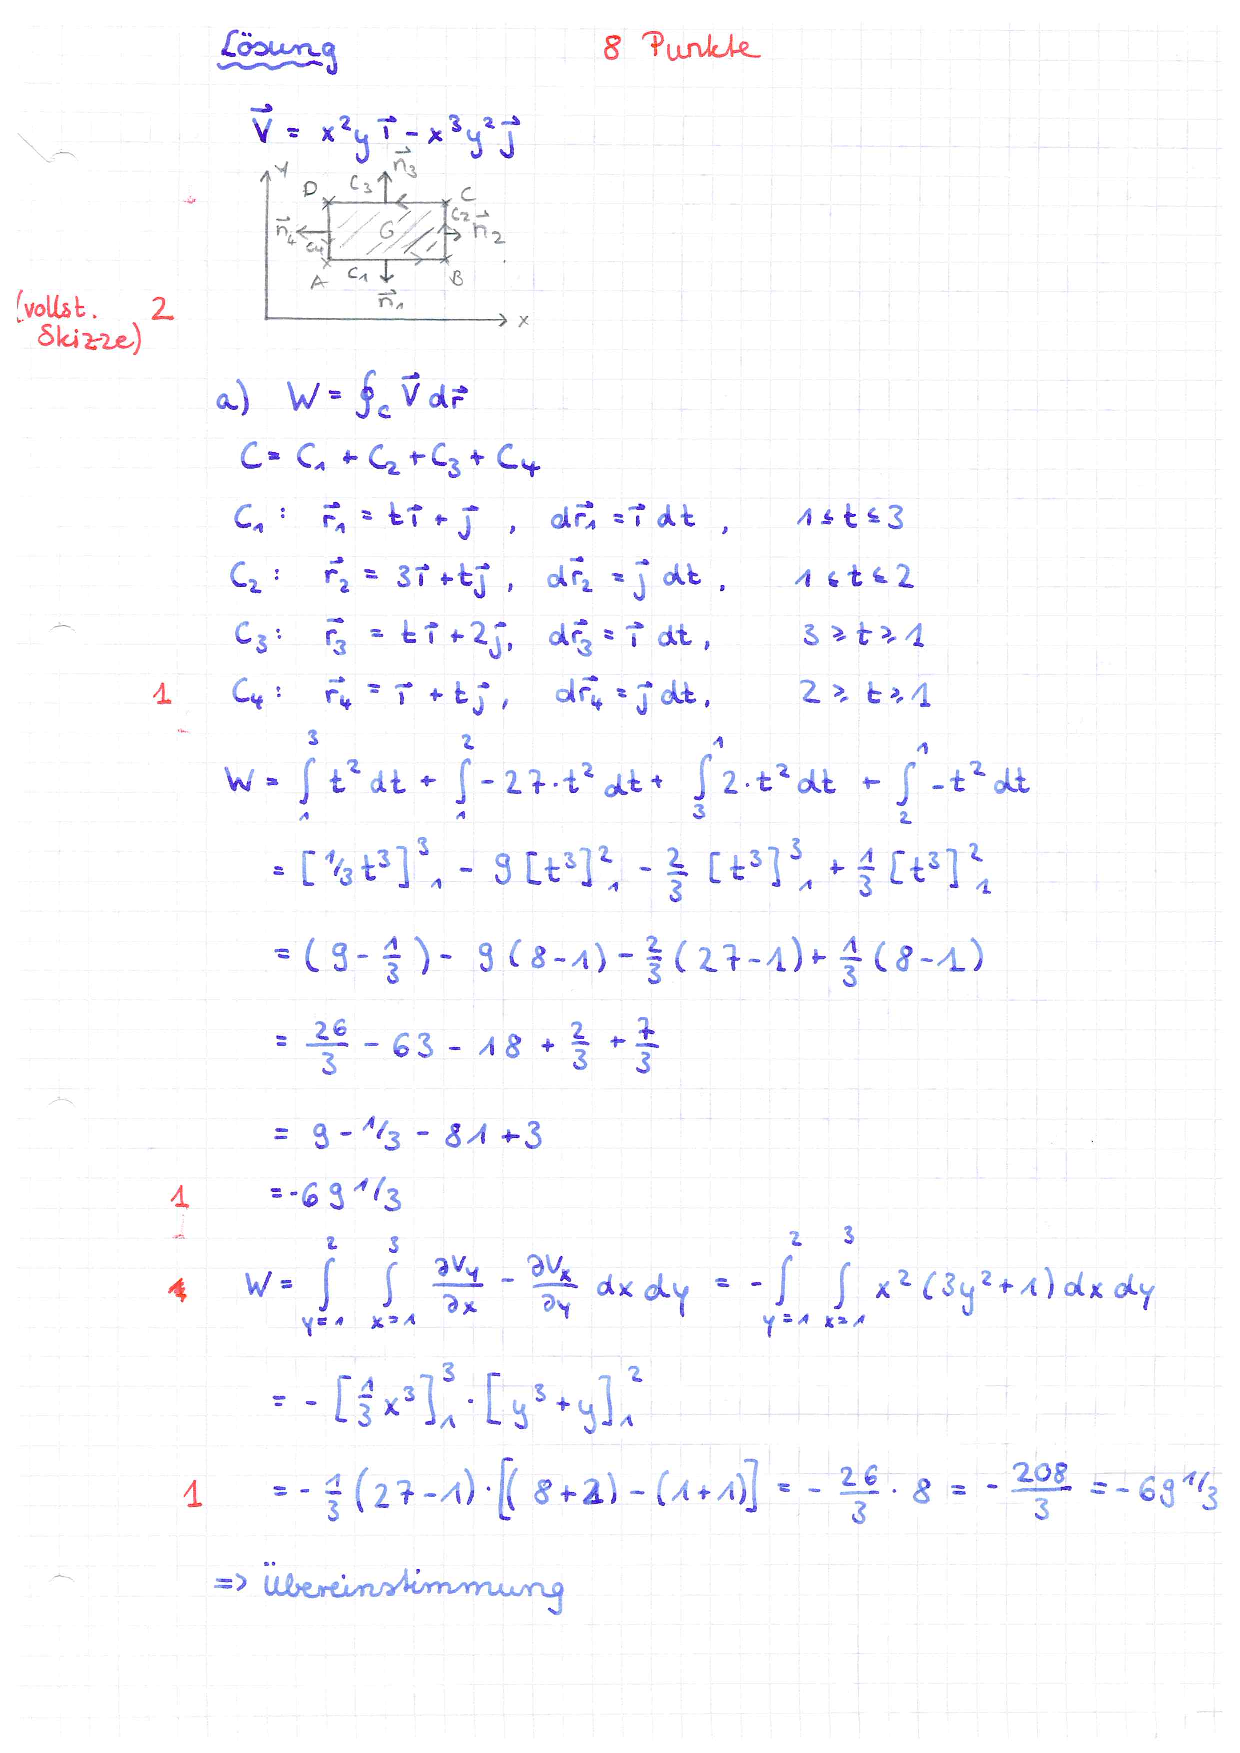
\includepdf[pages=-]{solution-stokes2D.pdf}
\end{atiSolution}